\documentclass[12pt]{article}
\usepackage{amsmath}
\usepackage{graphicx, float} % Required for inserting images
\usepackage[english]{babel}
\usepackage{amsthm}
\usepackage{amssymb}
% \usepackage{fullpage}
\usepackage[a4paper, right = 0.8in, left = 0.8in, top=0.5in, bottom = 0.2in]{geometry}
\usepackage[protrusion=true,expansion=true]{microtype}	
\usepackage{pgfplots}

\usepackage{subfiles}

\pgfplotsset{width=10cm,compat=1.9}
\usepgfplotslibrary{external}
\tikzexternalize

\newtheorem{theorem}{Theorem}[section]
\newtheorem{corollary}{Corollary}[theorem]
\newtheorem{lemma}[theorem]{Lemma}

\theoremstyle{definition}
\newtheorem{definition}{Definition}[section]

\theoremstyle{definition}
\newtheorem{example}{Example}[section]

\theoremstyle{remark}
\newtheorem*{remark}{Remark}

% \renewcommand\qedsymbol{$\blacksquare$} // For QED symbol

\begin{document}

\title{LS2102: BIOLOGY LABORATORY III\\[2ex] LAB REPORT}
\author{Ronit Bhuyan \\Roll No. 22MS025}
\date{$8^{th}$ August 2023}

\maketitle

\section*{Aim}
Determination of column Void Volume/Dead volume using gel-filtration chromatography.

\section*{Theory}
Gel filtration is also known as size-exclusion chromatography or molecular-sieve chromatography. In this process, separation of molecules is based on the differing ability of molecules in the sample to enter the pores of the gel-filtration medium because of their differing sizes.The uses of Gel Filtration chromatography thus include separation of polysaccharides, nucleic acids,etc in an aqueous medium as well as determination of molecular weights of various proteins.



\section*{Procedure}
1.Initially,the gel filtration column was filled with Sephadex G-75(Stationary Phase). The bed volume for our experiment was 49.5 mL.\\
\\
2.Now blue dextran dye of volume 990 \textmu L was filled into the column with the help of a micropipette. The volume of Blue Dextran should ideally be 2-3 \% of the Bed volume.\\
\\
3.A buffer composed of 50mM tris-HCl and 100mM NaOH was added to it.\\
\\
4.After adding the buffer, the stopcock was removed and the elute was collected in a 15mL tube until the first appearence of the blue dye. Care should be taken to regularly replenish the column with the buffer so that it doesn't run dry. \\
\\
5.After the initial appearence of the dye from the column, 0.5 mL of it was collected in different tubes. This process is repeated until all the blue dye comes out.\\
\\
6.Then 0.5 mL  of buffer was added to each tube and its absorbance was calculated at 610 nm using a spectrometer. The buffer was added so that the Absorbance remains in the Beer-Lambart's range.
(A blank test tube consisting of only the buffer was taken as the reference with respect to which the other Absorbances were calculated.)\\

\pagebreak


\section*{Observations and Data}

The following absorbance values were calculated at 610 nm for different test tubes.

\begin{table}[H]
   \centering
    \begin{tabular}{|c|c|}
    \hline
    \textbf{Tube No.} & \textbf{Absorbance}\\
    \hline
      1   & 0.073 \\
      \hline
       2  & 0.291\\
       \hline
       3  & 0.463\\
       \hline
       4  & 0.660\\
       \hline
       5  & 0.876\\
       \hline
       6  & 1.019\\
       \hline
       7  & 0.940\\
       \hline
       8  & 0.894\\
       \hline
       9  & 0.757\\
       \hline
       10 & 0.618\\
       \hline
       11  & 0.491\\
       \hline
       12  & 0.357\\
      \hline
    \end{tabular}
    \caption{Absorbance of Different Samples}
    \label{tab:my_label}
\end{table}

Using the above Absorbance values, a graph depicting the absorbance values of test tubes was plotted.

\begin{figure}[H]
    \centering
    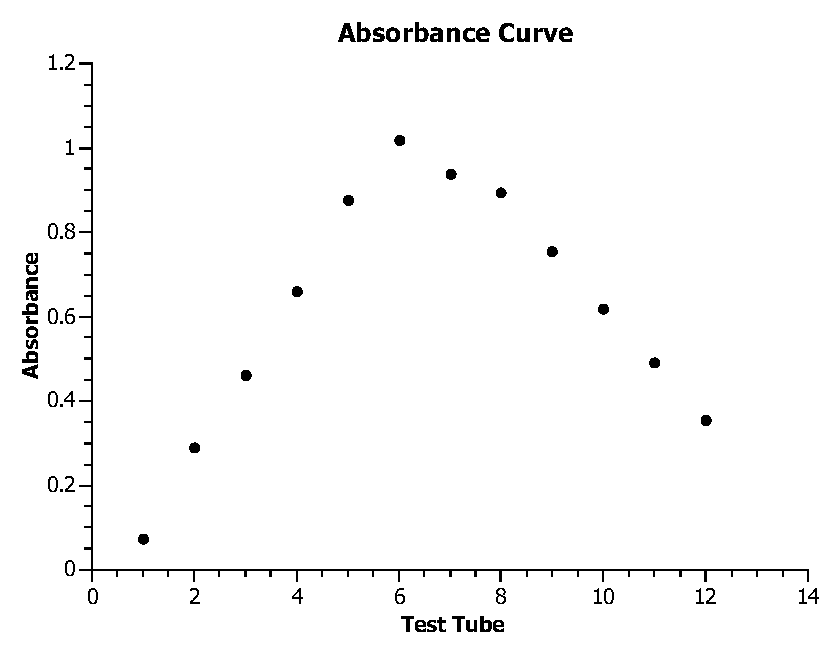
\includegraphics{Graph4.eps}
    \caption{Absorbance Curve at 610 nm}
    \label{fig:enter-label}
\end{figure}

\pagebreak
\section*{Calculations}


The collected volume of the buffer initially = 16mL\\
\\
From the graph it is clear that the maximum absorbance was observed in test tube no. 6
Hence the dye volume with respect to this tube number is 
  6*0.5=3 mL\\
\\So, Void Volume of the column is 3+16=19 mL.\\


\section*{Conclusions}
So using the Gel-chromatography,we successfully determined the Void/Dead Volume($V_{0}$) of the column to be \textbf{19mL} (Sum of the volume of buffer collected and the volume of the dye at which maximum absorbance occurs.)




\end{document}
